\chapter{まとめと今後の展望}
\section{まとめ}
X線CTは人体を切開することなく人体内部の状態を観察することができる、現代医療の画像診断の根幹をなす重要技術であり、年々その検査件数は増加し、適応範囲も拡大している。しかしそれに伴い、医療被ばくに占めるCTの割合が増加傾向にあることが指摘されており。特に日本においてはCTの普及率が諸外国に比べて圧倒的に高く、今後超高齢化社会を迎えCTの需要はより一層拡大し、医療被ばくの問題が増々深刻化すると考えられ、CTの低被ばく化は昨今の医療技術において最重要課題となっている。また、CT値のみを一つのパラメーターとする「単色画像」はCT誕生当時から課題であり、それにより物質同定が困難であったり、ビームハードニングアーチファクトが生じるなど、臨床現場において画像診断に制限を与えており、この問題が解決されること画像診断の幅が大きく広がり様々な病気の早期発見つながることも期待される。\\
本研究では、$\sim100万$という非常に大きい内部増幅機能をもつ半導体光素子であるMPPCを用いた「低被ばく」かつ「多色」撮影が可能な革新的X線CTシステムを考案し、従来のX線CTとの比較を行った。CTの画像評価において最も基本的かつ重要な画像ノイズ・低コントラスト分解能・空間分解能の評価を超低線量下で行った。その結果、すべての評価項目に置いて、MPPCでは従来型CTのPDによりも同じ線量でも圧倒的に優れた結果が得られ、MPPCを用いることで、低線量下でもPDと同等以上に高い画像S/Nを実現できることが実証できた(第6章)。これより被ばく量の問題により使用が制限されてきた子供や妊婦といった患者にも、X線CTによる内部撮影が可能になると期待できる。従来CTの光検出部をMPPCに変えるだけで実現できるため、本研究は早期における臨床応用・実現の点でも非常に優れているといえる。
また、線量自体を1/200に下げることができれば、フォトンカウンティングCTの障壁とされてきた高レートの問題を解決することができ、個々のX線パルスについてエネルギーの取得も容易となる(第7章)。たとえて言うならば、”白黒テレビがカラーテレビになる” ほど情報量の増加が見込め、様々な多色イメージングが期待される。その一例として、本研究では「コントラストの強調」「ビームハードニングアーチファクトの低減」「物質同定」「K-edgeイメージング」といった多色イメージングを行い、その有用性も検証できた。


\section{今後の展望}
本研究は、もっとも単純な$1\times1$mm$^^2$のMPPC単素子による検証実験を行ったが、今後はより実用的なCTシステムへの拡張を考えている。現在進めているのは16チャンネルの1次元MPPCアレイを専用アナログ・デジタルLSIを用いた、「多色マルチスライスX線モジュール」の開発である。これまでは単素子で撮影を行っていたため、シングルスライス撮影しかできなかったが、この16チャンネルアレイを用いることでマルチスライスが可能となり、MPPCアレイを用いた「低被ばく」かつ「多色」という世界で類を見ないCTとなることが期待される。\\

また、その先の展望としてはMPPCを1次元から2次元にアレイ化し、我々がこれまで開発した高精細シンチレータと組み合わせたX線モジュールの開発も考えている。これまで、YAPシンチレータ同様にフォトンカウンティングに有効なCe;GAGG シンチレータのプレートに0.25-mm ピッチでダイシング加工を施し、8×8 MPPCアレイと組み合わせることで0.3 mmの空間分解能を実現している。また、わずか4chの出力信号を用いて31, 60, 88keVの$\gamma$線を用いた「3色イメージング」にも成功した(\Fref{fig:oshimaetal})。この高精細シンチレータと2次元MPPCアレイを組み合わせ、CTモジュールを作成することでさらに進化した「多色」かつ「低線量」のマルチスライスCTへと発展が可能である。このような高精細シンチレータを用いた低被ばくCTは、簡便かつ低コスト、また既存のCTの置き換えも容易であり、今後のCT業界にブレークスルーを起こすことも期待できる。現在は怪我をしたときや健康診断の画像診断の入り口はレントゲンなどの一般撮影であるが、一般撮影レベルの被ばく量でCT撮影が可能となればCTも検査の入口として手軽に撮影することが可能になり、病気の早期発見につながる。このように「低被ばく」と「多色化」が切り拓く新たな画像診断の可能性は無限である。本研究が全世界のCTメーカーにCTの変革の可能性を示唆し、新たなCT画像診断の可能性を切り拓く、一石となることを願っている。



\begin{figure}[H]
 \begin{center}
 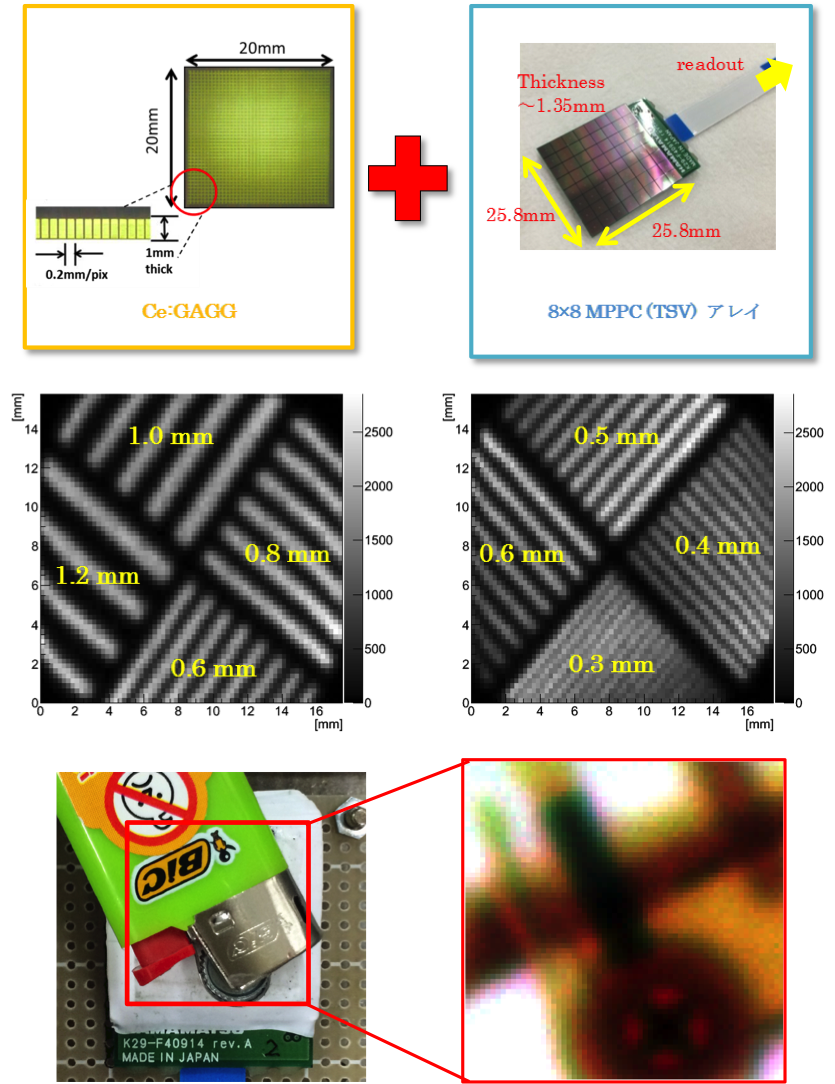
\includegraphics[bb=0.000000 0.000000 400.766870 520.276990,width=1\hsize]{image2/chapter5/oshimaetal.png} 
 \end{center}
 \caption{高精細シンチレータ(GAGG)とMPPCの外観とイメージング結果\cite{oshima_etal}}
 \label{fig:oshimaetal}
\end{figure}
